\documentclass[12pt]{article}
\usepackage[margin=1.5cm]{geometry}
\usepackage{parskip}
\usepackage{amsmath}
\usepackage{amssymb}
\usepackage{amsfonts}
\usepackage{enumitem}
\usepackage{graphicx}
\usepackage{stmaryrd}
\graphicspath{ {./images/} }


\begin{document}
\begin{enumerate}[label=(\alph*)]

  \item
    A procedure's flowgraph is a graph constructed of basic blocks that represent the possible control flow paths that an execution of the procedure could take.

    A basic block is a maximally large set of sequential instructions that has no entry points except the first instruction, and no exit points except for the final instruction.

    Flowgraph construction is made imprecise by indirect jumps, i.e. where the destination of a jump is decided by a value in a register for example. In general, it is impossible to know the values in registers at compile-time, so we are unable to always know the exact locations that an indirect jump can lead to.

  \item
    In a flowgraph, a node $n$ dominates another node $n'$ if in order to execute $n'$ we must have executed $n$.

    Strict dominance requires that $n \neq n'$, as well as domination.

    From a flowgraph, we can use strict dominance (more specifically, immediate dominance, which requires that we do not dominate any other strict dominator of the dominated node) as a relation to create edges, which generates a dominance tree.

    The dominance frontier of a node $n$ is the set of nodes that are not strictly dominated by $n$, but have an immediate predecessor dominated by $n$.

  \item
    We define data-flow equations as follows:

    $in-dom(n) = \begin{cases}\bigcap_{p \in pred(n)} out-dom(p) & pred(n) \neq \{\}\\\{\} & \text{otherwise}\end{cases}$

    $out-dom(n) = in-dom(n) \setminus kill(n) \cup gen(n)$

    Where $kill(n)$ is the empty set, since dominance is only killed based on the predecessors of a node (implicitly computed in $in-dom(n)$), and $gen(n) = \{n\}$.

    Then, we combine them (expanding $kill$ and $gen$):

    $dom(n) = \begin{cases}(\bigcap_{p \in pred(n)} dom(p)) \cup \{n\} & pred(n) \neq \{\}\\\{n\} & \text{otherwise}\end{cases}$

    We then give the following algorithm for computing dominance:

\begin{verbatim}
dom[0] = {0}
dom[1..n] = U
while (dom[] changes) do
  for i in 1..n do
    dom[i] = big_intersect(p in pred(n), dom[p]) U {i}
\end{verbatim}

\item
  Dominance can find loops in a flowgraph if we have an edge in our flowgraph from $n$ to $n'$, where $n'$ dominates $n$.

\item
  SSA form is the form of a program where each variable is statically assigned to a value at most once.

\item


  We compute the following flowgraph:

  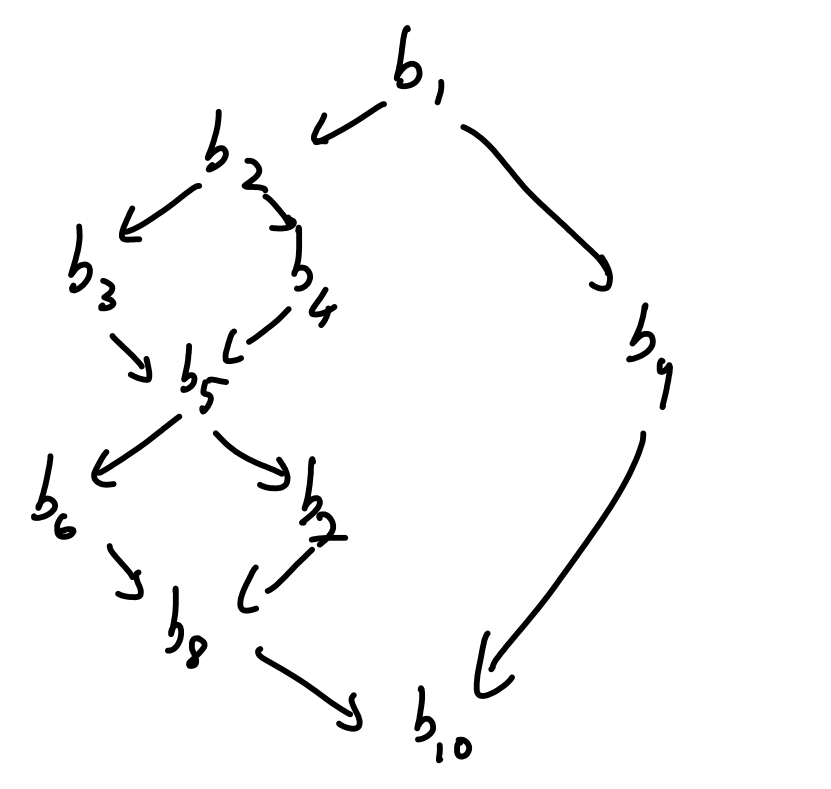
\includegraphics[scale=0.3]{flowgraph}

  We compute the following dominance tree:

  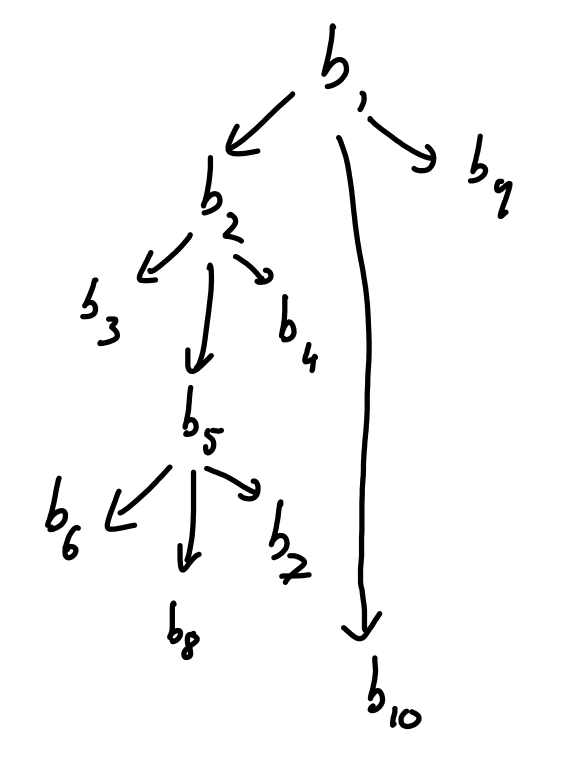
\includegraphics[scale=0.3]{dominance}

  We see that we should insert a $\phi$ node at the start of a block if it in the dominance frontier of another node.

  We get dominance frontiers:

\begin{verbatim}
b1: {}
b2: {b10}
b3: {b5}
b4: {b5}
b5: {b10}
b6: {b8}
b7: {b8}
b8: {b10}
b9: {b10}
b10: {}
\end{verbatim}

So we insert $phi$ nodes in \texttt{b5}, \texttt{b8}, and \texttt{b10} as follows:

\begin{verbatim}
b1:  LDR x1, #0xFF00
     LDR y1, #0xFF08
     BEQ x1, #0, b9
b2:  BEQ x1, #1, b4
b3:  ADD x2, x1, #2
     BR  b5
b4:  ADD x3, x2, y1
b5:  x4 = phi(x2, x3) 
     BEQ x4, #8, b7
b6:  STR x4, #0xFFA0
     BR  b8
b7:  STR y1, #0xFFA0
b8:  x5 = phi(x4, x4)
     ADD x6, x5, y1
     BR  b10
b9:  ADD y2, y1, #1
b10: x7 = phi(x1, x5)
     y3 = phi(y1, y2)
     ADD x8, x7, #1
     STR x8, #0xFF00
\end{verbatim}





        
    \end{enumerate}
\end{document}
